%! Author = melek
%! Date = 22.01.2023

% Preamble
\documentclass[11pt]{article}

% Packages
\usepackage{amsmath}
\usepackage{graphicx}
\graphicspath{ {../images/} }

\title{Assignment 3: Q-Learning and Actor-Critic Algorithms}
\author{huseyinabanox@gmail.com}
\date{January 2023}

% Document
\begin{document}

    \maketitle

    \section{Part 1: Q-Learning}

    \subsection*{Question 1: basic Q-learning performance (DQN)}

    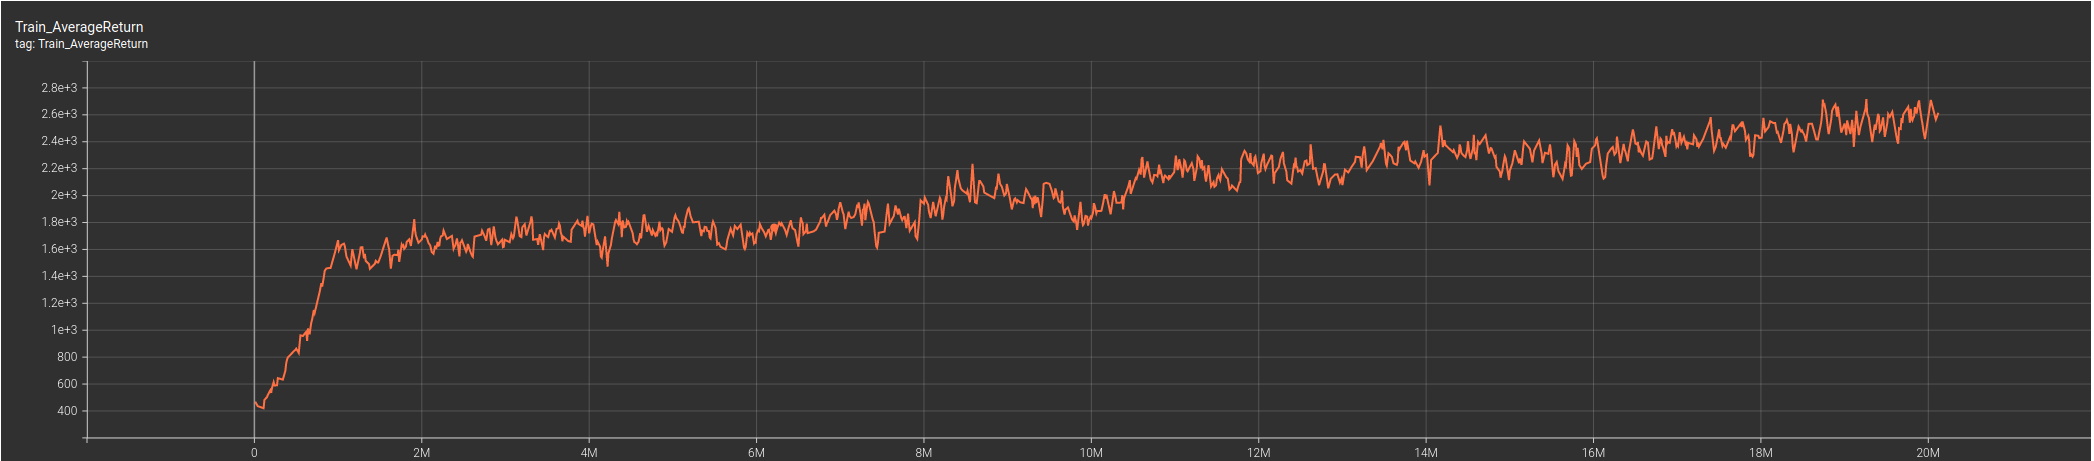
\includegraphics[scale=0.8]{q1/packman-20M}

    After 20M iterations the learning curve looks like above.
    It is taken from tensorboard.
    Relevant log files can be found under data folder.

    Double Q network obtains better returns, as expected.

    \subsection*{Question 2: double Q-learning (DDQN)}

    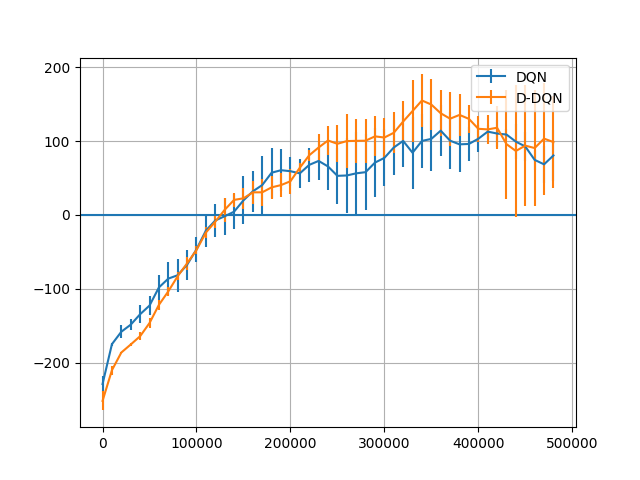
\includegraphics[scale=0.8]{q2/q2}

    LunarLander-v3 environment is used for 3 seeds per configuration e.g. DQN vs D-DQN as stated in the question.
    Different seed results are averaged and the plot above is generated.
    combine\_results\_q2.py file is used to combine results.

    \subsection*{Question 3: experimenting with hyperparameters}

    TODO: solve this question

    \section{Part 2: Actor-Critic}

    \subsection*{Question 4: Sanity check with Cartpole}

    Actor critic algorithm is tested in cartpole environment.
    Different target update parameters and gradient steps parameters are tried.

    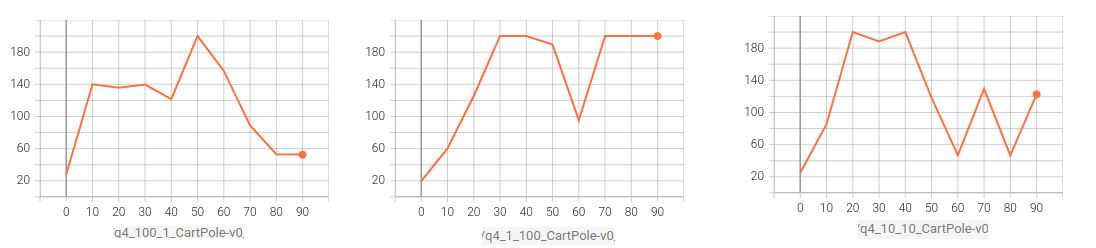
\includegraphics[scale=1.5]{q4/q4}.

    Subtitles show the used parameters.

    Best performance is obtained when both parameters are set to 10.
    If target update is set to 1 and gradient steps are set to 100, learning seems to be more stable.
    This results shows the importance of gradient steps.

    \subsection*{Question 5: Run actor-critic with more difficult tasks}

    Best results are obtained when both parameters are set to 10.

    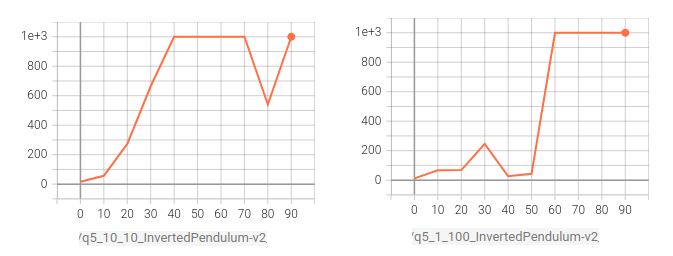
\includegraphics[scale=2]{q5/q5_inverted_pendulum}.

    After 100 iterations, InvertedPendulum return is around 1000, as expected.
    After 20 iterations, InvertedPendulum return should is above 100, as expected.

    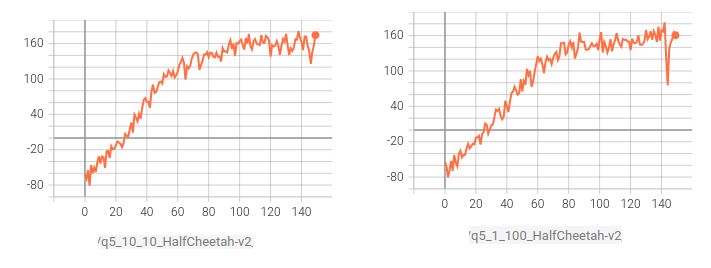
\includegraphics[scale=2]{q5/q5_half_cheetah}.

    After 150 iterations, HalfCheetah return is around 150, as expected.
    After 20 iterations, HalfCheetah return should is above -40, as expected.

    \section{Part 3: Soft Actor-Critic}

    \subsection*{Question 6: Run soft actor-critic more difficult tasks}

    Actor updates and critic updates are set to 10.

    After 20000 steps, InvertedPendulum return is expected to reach 1000.
    Actually it is reached after 9k steps.

\end{document}